\documentclass{article}
\usepackage[top=2cm,bottom=2cm,left=1.5cm,right=1.5cm]{geometry}
\usepackage[utf8]{inputenc}
\usepackage[utf8]{vietnam}
\usepackage[unicode=true]{hyperref}
\usepackage{minted}
\usepackage{enumitem}
\usepackage{booktabs}
\usepackage{amssymb}
\usepackage{multirow}
\usepackage{placeins}
\usepackage{indentfirst}

\usepackage{tikz}
\usetikzlibrary{arrows.meta}
\usetikzlibrary{positioning}
\usetikzlibrary{shapes.geometric}

\renewcommand{\familydefault}{\sfdefault}
\setlist[itemize]{topsep=0pt,itemsep=0pt}
\setlist[enumerate]{topsep=0pt,itemsep=0pt}
\newcommand{\completedpath}{\textit{Completed path}}

\title{\bf Kiểm thử luồng dữ liệu $-$ 2021II INT3117 1}
\author{Ngô Quang Dương/17020191}
\date{\today}

\begin{document}

\maketitle

\section{Chương trình đăng nhập}

\par GitHub Repository: \url{https://github.com/duong755/INT3117_1_2021II}

\begin{minted}[linenos,frame=single,framesep=10pt,breaklines]{js}
var EMAIL_REGEX = /(emailregex)/; // too long to write down here
var signInForm = document.forms[0];
signInForm.addEventListener('submit', function (submitEvent) {
  submitEvent.preventDefault();
  var email = document.querySelector('.text-field.email input').value;
  var password = document.querySelector('.text-field.password input').value;
  var emailError = '';
  var passwordError = '';
  if (email.trim() === '') {
    emailError = 'Không được để trống email';
  } else if (!EMAIL_REGEX.test(email)) {
    emailError = 'Email không hợp lệ';
  } else if (email.trim().length > 320) {
    emailError = 'Email không được dài quá 320 kí tự';
  } else {
    emailError = '';
  }
  if (password.trim() === '') {
    passwordError = 'Không được để trống mật khẩu';
  } else {
    passwordError = '';
  }
  var emailErrorContainer = document.querySelector('.text-field.email .error-message');
  var passwordErrorContainer = document.querySelector('.text-field.password .error-message');
  emailErrorContainer.innerHTML = emailError;
  passwordErrorContainer.innerHTML = passwordError;
  if (emailError === '' && passwordError === '') {
    this.submit(); // `this` is `signInForm`
  }
});
\end{minted}

\section{Các biến trong chương trình, đồ thị luồng dữ liệu}

\par Chương trình trên sử dụng các biến sau (ở đây không nêu ra biến toàn cục \texttt{document}):
\bigskip
\begin{enumerate}[label = (v\arabic*)]
    \item \texttt{EMAIL\_REGEX}
    \item \texttt{signInForm}
    \item \texttt{submitEvent}
    \item \texttt{email}
    \item \texttt{password}
    \item \texttt{emailError}
    \item \texttt{passwordError}
    \item \texttt{emailErrorContainer}
    \item \texttt{passwordErrorContainer}
\end{enumerate}

\bigskip
\par Dựa vào đồ thị luồng dữ liệu (hình~\ref{fig:data-flow-graph}), ta xác định được 16 đường đi đầy đủ có thể có như sau:
\bigskip

\begin{enumerate}[label = (\arabic*),itemindent=1cm]
    \item 1--8, 9 (T), 10, 16 (T), 17, 19, 20, 21, 22, 23 (T), 24
    \item 1--8, 9 (T), 10, 16 (T), 17, 19, 20, 21, 22, 23 (F)
    \item 1--8, 9 (T), 10, 16 (F), 18, 19, 20, 21, 22, 23 (T), 24
    \item 1--8, 9 (T), 10, 16 (F), 18, 19, 20, 21, 22, 23 (F)
    \item 1--8, 9 (F), 11 (T), 12, 16 (T), 17, 19, 20, 21, 22, 23 (T), 24
    \item 1--8, 9 (F), 11 (T), 12, 16 (T), 17, 19, 20, 21, 22, 23 (F)
    \item 1--8, 9 (F), 11 (T), 12, 16 (F), 18, 19, 20, 21, 22, 23 (T), 24
    \item 1--8, 9 (F), 11 (T), 12, 16 (F), 18, 19, 20, 21, 22, 23 (F)
    \item 1--8, 9 (F), 11 (F), 13 (T), 14, 16 (T), 17, 19, 20, 21, 22, 23 (T), 24
    \item 1--8, 9 (F), 11 (F), 13 (T), 14, 16 (T), 17, 19, 20, 21, 22, 23 (F)
    \item 1--8, 9 (F), 11 (F), 13 (T), 14, 16 (F), 18, 19, 20, 21, 22, 23 (T), 24
    \item 1--8, 9 (F), 11 (F), 13 (T), 14, 16 (F), 18, 19, 20, 21, 22, 23 (F)
    \item 1--8, 9 (F), 11 (F), 13 (F), 15, 16 (T), 17, 19, 20, 21, 22, 23 (T), 24
    \item 1--8, 9 (F), 11 (F), 13 (F), 15, 16 (T), 17, 19, 20, 21, 22, 23 (F)
    \item 1--8, 9 (F), 11 (F), 13 (F), 15, 16 (T), 18, 19, 20, 21, 22, 23 (T), 24
    \item 1--8, 9 (F), 11 (F), 13 (F), 15, 16 (T), 18, 19, 20, 21, 22, 23 (F)
\end{enumerate}

\bigskip
\bigskip
\bigskip
\par Dựa vào sơ đồ luồng dữ liệu, bảng~\ref{table:variable-usage} thống kê các kiểu sử dụng của từng biến:
\bigskip
\bigskip
\bigskip

\FloatBarrier
\begin{table}[htp]
    \centering
    % chktex-file 44
    \begin{tabular}{l|c|c|c}
        \texttt{Variable}                    & def                        & p-use                 & c-use      \\
        \toprule
        \bottomrule
        \texttt{EMAIL\_REGEX} (v1)           & \{ 1 \}                    & \{ 11 \}              & $\varnothing$           \\
        \hline
        \texttt{signInForm} (v2)             & \{ 2 \}                    & $\varnothing$         & \{ 3, 24 \}             \\
        \hline
        \texttt{submitEvent} (v3)            & \{ 3 \}                    & $\varnothing$         & \{ 4 \}                 \\
        \hline
        \texttt{email} (v4)                  & \{ 5 \}                    & \{ 9, 11, 13 \}       & $\varnothing$           \\
        \hline
        \texttt{password} (v5)               & \{ 6 \}                    & \{ 16 \}              & $\varnothing$           \\
        \hline
        \texttt{emailError} (v6)             & \{ 7, 10, 12, 14, 15 \}    & \{ 23 \}              & \{ 21 \}                \\
        \hline
        \texttt{passwordError} (v7)          & \{ 8, 17, 18 \}            & \{ 23 \}              & \{ 22 \}                \\
        \hline
        \texttt{emailErrorContainer} (v8)    & \{ 19 \}                   & $\varnothing$         & \{ 21 \}                \\
        \hline
        \texttt{passwordErrorContainer} (v9) & \{ 20 \}                   & $\varnothing$         & \{ 22 \}                \\
    \end{tabular}
    \caption{Bảng các biến và các dòng sử dụng chúng}
    {\label{table:variable-usage}}
\end{table}
\FloatBarrier

\begin{figure}[htp]
    \centering
    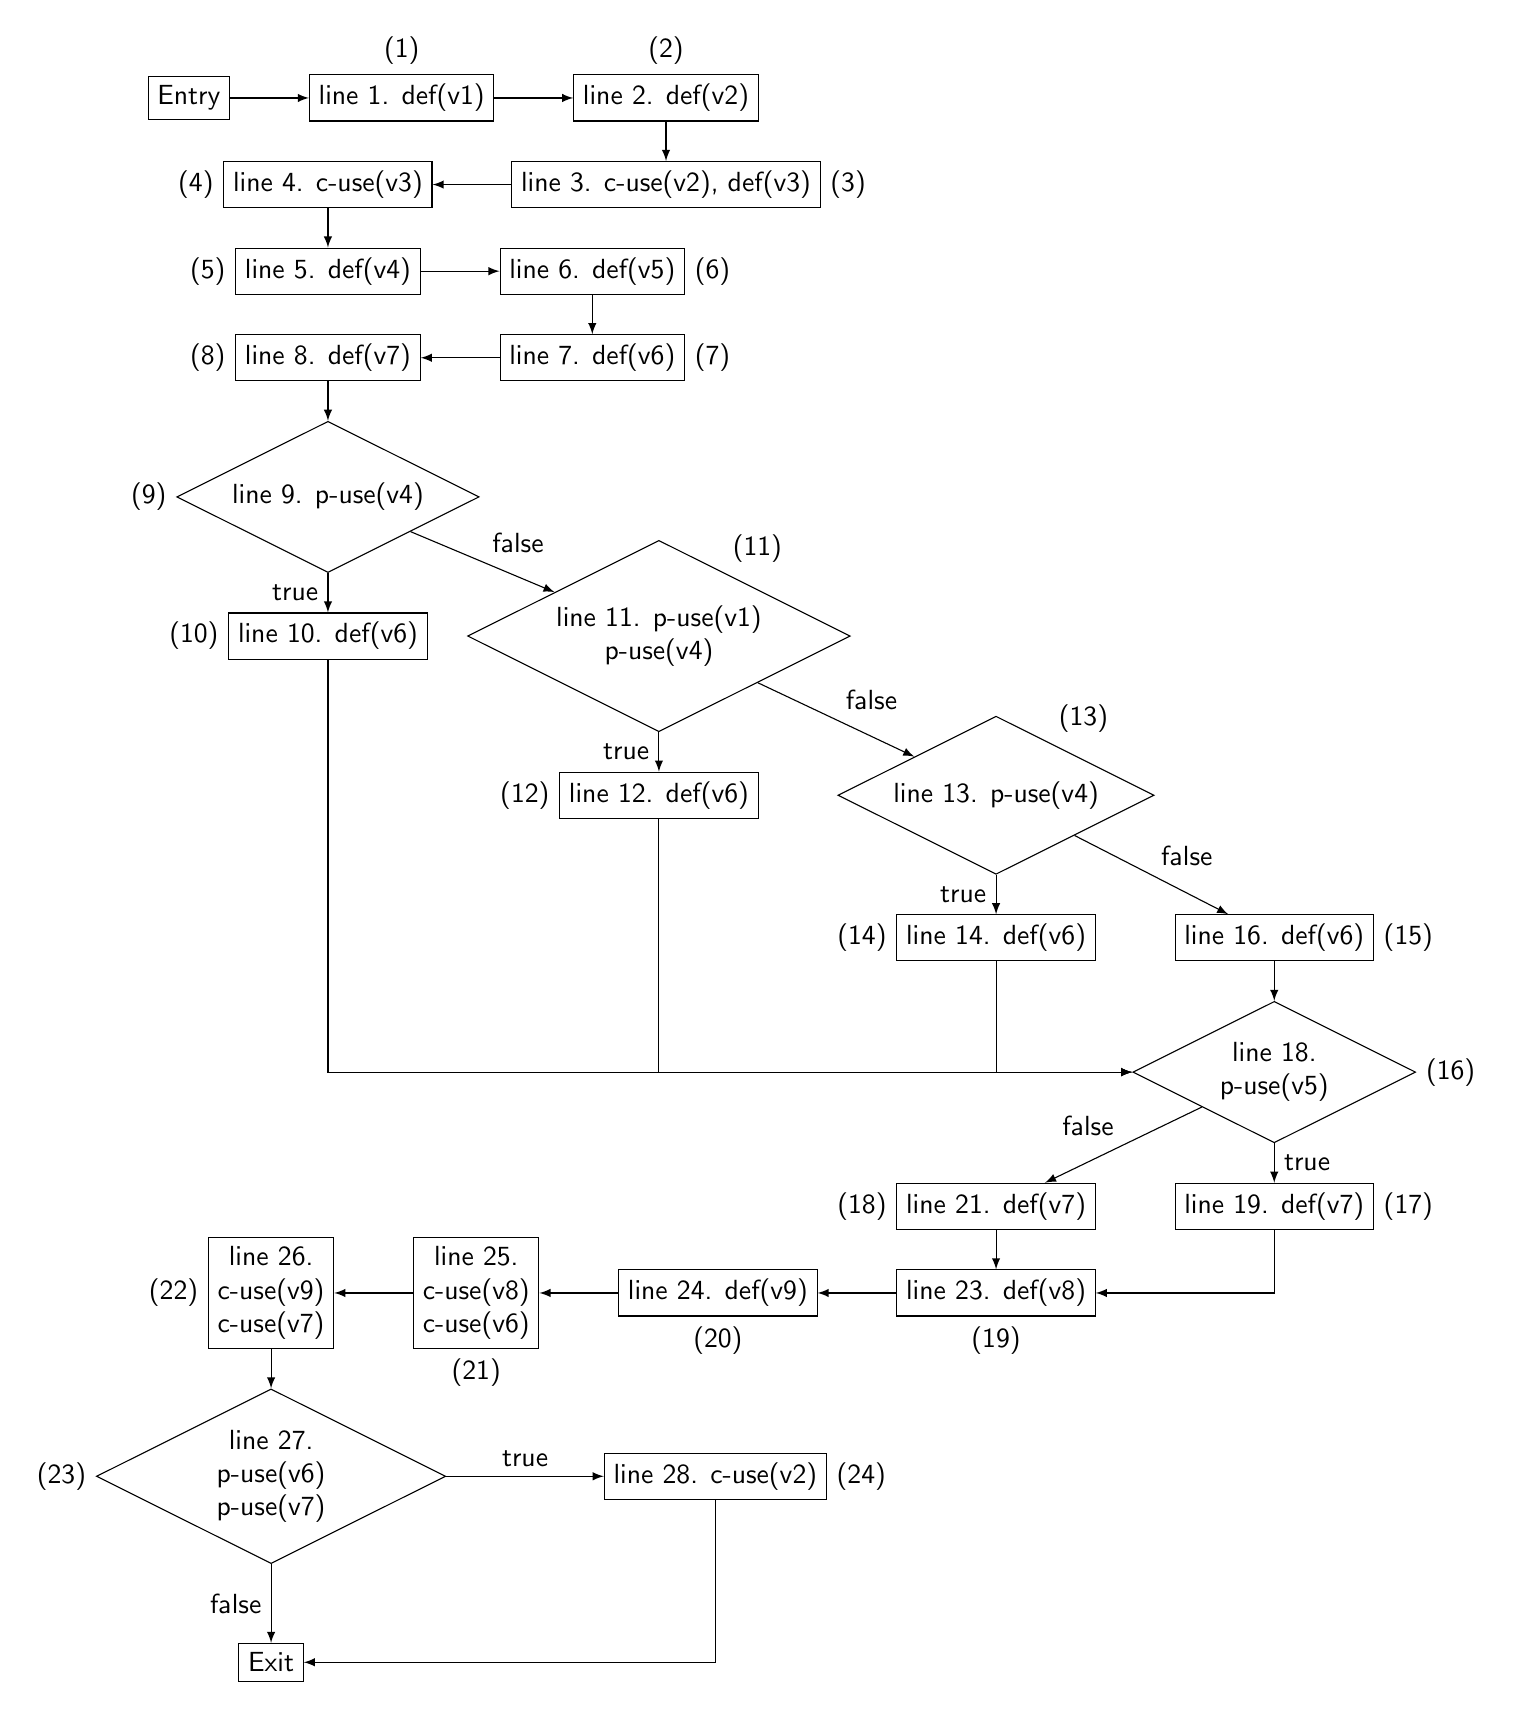
\begin{tikzpicture}[
            every node/.style={rectangle,draw,align=center},
            label node/.style={rectangle,draw=none},
            level 1/.style={level distance=1cm},
            level 3/.style={sibling distance=3cm}
        ]
        \tikzset{>=latex}
        \node (entry) {Entry};
        \node [right=of entry,label={above:(1)}] (node 1) {line 1. def(v1)};
        \node [right=of node 1,label={above:(2)}] (node 2) {line 2. def(v2)};
        \node [below=0.5cm of node 2,label={right:(3)}] (node 3) {line 3. c-use(v2), def(v3)};
        \node [left=of node 3,label={left:(4)}] (node 4) {line 4. c-use(v3)};
        \node [below=0.5cm of node 4,label={left:(5)}] (node 5) {line 5. def(v4)};
        \node [right=of node 5,label={right:(6)}] (node 6) {line 6. def(v5)};
        \node [below=0.5cm of node 6,label={right:(7)}] (node 7) {line 7. def(v6)};
        \node [left=of node 7,label={left:(8)}] (node 8) {line 8. def(v7)};
        \node [below=0.5cm of node 8,label={left:(9)},diamond,aspect=2] (node 9) {line 9. p-use(v4)};
        \node [below=0.5cm of node 9,label={left:(10)}] (node 10) {line 10. def(v6)};
        \node [right=0.5cm of node 10,label={above right:(11)},diamond,aspect=2] (node 11) {line 11. p-use(v1) \\ p-use(v4)};
        \node [below=0.5cm of node 11,label={left:(12)}] (node 12) {line 12. def(v6)};
        \node [right=of node 12,label={above right:(13)},diamond,aspect=2] (node 13) {line 13. p-use(v4)};
        \node [below=0.5cm of node 13,label={left:(14)}] (node 14) {line 14. def(v6)};
        \node [right=of node 14,label={right:(15)}] (node 15) {line 16. def(v6)};
        \node [below=0.5cm of node 15,label={right:(16)},diamond,aspect=2] (node 16) {line 18.\\ p-use(v5)};
        \node [below=0.5cm of node 16,label={right:(17)}] (node 17) {line 19. def(v7)};
        \node [left=of node 17,label={left:(18)}] (node 18) {line 21. def(v7)};
        \node [below=0.5cm of node 18,label={below:(19)}] (node 19) {line 23. def(v8)};
        \node [left=of node 19,label={below:(20)}] (node 20) {line 24. def(v9)};
        \node [left=of node 20,label={below:(21)}] (node 21) {line 25.\\ c-use(v8)\\ c-use(v6)};
        \node [left=of node 21,label={left:(22)}] (node 22) {line 26.\\ c-use(v9)\\ c-use(v7)};
        \node [below=0.5cm of node 22,label={left:(23)},diamond,aspect=2] (node 23) {line 27.\\ p-use(v6)\\ p-use(v7)};
        \node [right=2cm of node 23,label={right:(24)}] (node 24) {line 28. c-use(v2)};
        \node [below=of node 23] (exit) {Exit};
        
        \draw[->] (entry) -- (node 1);
        \draw[->] (node 1) -- (node 2);
        \draw[->] (node 2) -- (node 3);
        \draw[->] (node 3) -- (node 4);
        \draw[->] (node 4) -- (node 5);
        \draw[->] (node 5) -- (node 6);
        \draw[->] (node 6) -- (node 7);
        \draw[->] (node 7) -- (node 8);
        \draw[->] (node 8) -- (node 9);
        \draw[->] (node 9) edge node[label node,left] {true} (node 10);
        \draw[->] (node 9) edge node[label node,above right] {false} (node 11);
        \draw[->] (node 11) edge node[label node,left] {true} (node 12);
        \draw[->] (node 11) edge node[label node,above right] {false} (node 13);
        \draw[->] (node 13) edge node[label node,left] {true} (node 14);
        \draw[->] (node 13) edge node[label node,above right] {false} (node 15);
        \draw[->] (node 15) -- (node 16);
        \draw[->] (node 16) edge node[label node,right] {true} (node 17);
        \draw[->] (node 16) edge node[label node,above left] {false} (node 18);
        \draw[->] (node 18) -- (node 19);
        \draw[->] (node 19) -- (node 20);
        \draw[->] (node 20) -- (node 21);
        \draw[->] (node 21) -- (node 22);
        \draw[->] (node 22) -- (node 23);
        \draw[->] (node 23) edge node[label node,above] {true} (node 24);
        \draw[->] (node 23) edge node[label node,left] {false} (exit);
        \draw[->] (node 10) |- (node 16);
        \draw[->] (node 12) |- (node 16);
        \draw[->] (node 14) |- (node 16);
        \draw[->] (node 17) |- (node 19);
        \draw[->] (node 24) |- (exit);
    \end{tikzpicture}
    \caption{Đồ thị luồng dữ liệu}
    {\label{fig:data-flow-graph}}
\end{figure}

\section{Kiểm thử}

\subsection{def-clear path}

\subsubsection*{\texttt{EMAIL\_REGEX} (v1)}

\begin{itemize}
    \item 1$-$8, 9 (F), 11
    \begin{itemize}
        \item \completedpath: (5), (6), (7), (8), (9), (10), (11), (12), (13), (14), (15), (16).
    \end{itemize}
\end{itemize}

\subsubsection*{\texttt{signInForm} (v2)}

\begin{itemize}
    \item 2, 3
    \begin{itemize}
        \item \completedpath: (1), (2), (3), (4), (5), (6), (7), (8), (9), (10), (11), (12), (13), (14), (15), (16)
    \end{itemize}
    \item 2--8, 9 (T), 10, 16 (T), 17, 19, 20, 21, 22, 23 (T), 24
    \begin{itemize}
        \item \completedpath: (1)
    \end{itemize}
    \item 2--8, 9 (T), 10, 16 (F), 18, 19, 20, 21, 22, 23 (T), 24
    \begin{itemize}
        \item \completedpath: (3)
    \end{itemize}
    \item 2--8, 9 (F), 11 (T), 12, 16 (T), 17, 19, 20, 21, 22, 23 (T), 24
    \begin{itemize}
        \item \completedpath: (5)
    \end{itemize}
    \item 2--8, 9 (F), 11 (T), 12, 16 (F), 18, 19, 20, 21, 22, 23 (T), 24
    \begin{itemize}
        \item \completedpath: (7)
    \end{itemize}
    \item 2--8, 9 (F), 11 (F), 13 (T), 14, 16 (T), 17, 19, 20, 21, 22, 23 (T), 24
    \begin{itemize}
        \item \completedpath: (9)
    \end{itemize}
    \item 2--8, 9 (F), 11 (F), 13 (T), 14, 16 (F), 18, 19, 20, 21, 22, 23 (T), 24
    \begin{itemize}
        \item \completedpath: (11)
    \end{itemize}
    \item 2--8, 9 (F), 11 (F), 13 (F), 15, 16 (T), 17, 19, 20, 21, 22, 23 (T), 24
    \begin{itemize}
        \item \completedpath: (13)
    \end{itemize}
    \item 2--8, 9 (F), 11 (F), 13 (F), 15, 16 (T), 18, 19, 20, 21, 22, 23 (T), 24
    \begin{itemize}
        \item \completedpath: (15)
    \end{itemize}
\end{itemize}

\subsubsection*{\texttt{submitEvent} (v3)}

\begin{itemize}
    \item 3, 4
    \begin{itemize}
        \item \completedpath: (1), (2), (3), (4), (5), (6), (7), (8), (9), (10), (11), (12), (13), (14), (15), (16)
    \end{itemize}
\end{itemize}

\subsubsection*{\texttt{email} (v4)}

\begin{itemize}
    \item 5$-$8, 9
    \begin{itemize}
        \item \completedpath: (1), (2), (3), (4), (5), (6), (7), (8), (9), (10), (11), (12), (13), (14), (15), (16)
    \end{itemize}
    \item 5$-$8, 9 (F), 11
    \begin{itemize}
        \item \completedpath: (5), (6), (7), (8), (9), (10), (11), (12), (13), (14), (15), (16)
    \end{itemize}
    \item 5$-8$, 9 (F), 11 (F), 13
    \begin{itemize}
        \item \completedpath: (9), (10), (11), (12), (13), (14), (15), (16)
    \end{itemize}
\end{itemize}

\subsubsection*{\texttt{password} (v5)}

\begin{itemize}
    \item 6, 7, 8, 9 (T), 10, 16
    \begin{itemize}
        \item \completedpath: (1), (2), (3), (4)
    \end{itemize}
    \item 6, 7, 8, 9 (F), 11 (T), 12, 16
    \begin{itemize}
        \item \completedpath: (5), (6), (7), (8)
    \end{itemize}
    \item 6, 7, 8, 9 (F), 11 (F), 13 (T), 14, 16
    \begin{itemize}
        \item \completedpath: (9), (10), (11), (12)
    \end{itemize}
    \item 6, 7, 8, 9 (F), 11 (F), 13 (F), 15, 16
    \begin{itemize}
        \item \completedpath: (13), (14), (15), (16)
    \end{itemize}
\end{itemize}

\subsubsection*{\texttt{emailError} (v6)}

\begin{itemize}
    \item 7, 8, 9
    \begin{itemize}
        \item \completedpath: (1), (2), (3), (4), (5), (6), (7), (8), (9), (10), (11), (12), (13), (14), (15), (16)
    \end{itemize}
    \item 7, 8, 9 (F), 11
    \begin{itemize}
        \item \completedpath: (5), (6), (7), (8), (9), (10), (11), (12), (13), (14), (15), (16)
    \end{itemize}
    \item 7, 8, 9 (F), 11 (F), 13
    \begin{itemize}
        \item \completedpath: (9), (10), (11), (12), (13), (14), (15), (16)
    \end{itemize}
    \item 10, 16 (T), 17, 19, 20, 21
    \begin{itemize}
        \item \completedpath: (1), (2)
    \end{itemize}
    \item 10, 16 (T), 17, 19, 20, 21, 22, 23
    \begin{itemize}
        \item \completedpath: (1), (2)
    \end{itemize}
    \item 10, 16 (F), 18, 19, 20, 21
    \begin{itemize}
        \item \completedpath: (3), (4)
    \end{itemize}
    \item 10, 16 (F), 18, 19, 20, 21, 22, 23
    \begin{itemize}
        \item \completedpath: (3), (4)
    \end{itemize}
    \item 12, 16 (T), 17, 19, 20, 21
    \begin{itemize}
        \item \completedpath: (5), (6)
    \end{itemize}
    \item 12, 16 (T), 17, 19, 20, 21, 22, 23
    \begin{itemize}
        \item \completedpath: (5), (6)
    \end{itemize}
    \item 12, 16 (F), 18, 19, 20, 21
    \begin{itemize}
        \item \completedpath: (7), (8)
    \end{itemize}
    \item 12, 16 (F), 18, 19, 20, 21, 22, 23 
    \begin{itemize}
        \item \completedpath: (7), (8)
    \end{itemize}
    \item 14, 16 (T), 17, 19, 20, 21
    \begin{itemize}
        \item \completedpath: (9), (10)
    \end{itemize}
    \item 14, 16 (T), 17, 19, 20, 21, 22, 23
    \begin{itemize}
        \item \completedpath: (9), (10)
    \end{itemize}
    \item 14, 16 (F), 18, 19, 20, 21
    \begin{itemize}
        \item \completedpath: (11), (12)
    \end{itemize}
    \item 14, 16 (F), 18, 19, 20, 21, 22, 23
    \begin{itemize}
        \item \completedpath: (11), (12)
    \end{itemize}
    \item 15, 16 (T), 17, 19, 20, 21
    \begin{itemize}
        \item \completedpath: (13), (14)
    \end{itemize}
    \item 15, 16 (T), 17, 19, 20, 21, 22, 23
    \begin{itemize}
        \item \completedpath: (13), (14)
    \end{itemize}
    \item 15, 16 (F), 18, 19, 20, 21
    \begin{itemize}
        \item \completedpath: (15), (16)
    \end{itemize}
    \item 15, 16 (F), 18, 19, 20, 21, 22, 23
    \begin{itemize}
        \item \completedpath: (15), (16)
    \end{itemize}
\end{itemize}

\subsubsection*{\texttt{passwordError} (v7)}

\begin{itemize}
    \item 8, 9 (T), 10, 16
    \begin{itemize}
        \item \completedpath: (1), (2), (3), (4)
    \end{itemize}
    \item 8, 9 (F), 11 (T), 12, 16
    \begin{itemize}
        \item \completedpath: (5), (6), (7), (8)
    \end{itemize}
    \item 8, 9 (F), 11 (F), 13 (T), 14, 16
    \begin{itemize}
        \item \completedpath: (9), (10), (11), (12)
    \end{itemize}
    \item 8, 9 (F), 11 (F), 13 (F), 15, 16
    \begin{itemize}
        \item \completedpath: (13), (14), (15), (16)
    \end{itemize}
    \item 17, 19, 20, 21, 22
    \begin{itemize}
        \item \completedpath: (9), (10), (13), (14)
    \end{itemize}
    \item 17, 19, 20, 21, 22, 23
    \begin{itemize}
        \item \completedpath: (9), (10), (13), (14)
    \end{itemize}
    \item 18, 19, 20, 21, 22
    \begin{itemize}
        \item \completedpath: (11), (12), (15), (16)
    \end{itemize}
    \item 18, 19, 20, 21, 22, 23
    \begin{itemize}
        \item \completedpath: (11), (12), (15), (16)
    \end{itemize}
\end{itemize}

\subsubsection*{\texttt{emailErrorContainer} (v8)}

\begin{itemize}
    \item 19, 20, 21
    \begin{itemize}
        \item \completedpath: (1), (2), (3), (4), (5), (6), (7), (8), (9), (10), (11), (12), (13), (14), (15), (16)
    \end{itemize}
\end{itemize}

\subsubsection*{\texttt{passwordErrorContainer} (v9)}

\begin{itemize}
    \item 20, 21, 22
    \begin{itemize}
        \item \completedpath: (1), (2), (3), (4), (5), (6), (7), (8), (9), (10), (11), (12), (13), (14), (15), (16)
    \end{itemize}
\end{itemize}

\subsection{du-pair}

\begin{enumerate}[label = (v\arabic*)]
    \item \texttt{EMAIL\_REGEX}: (1, 11)
    \item \texttt{signInForm}: (2, 3), (1, 24)
    \item \texttt{submitEvent}: (3, 4)
    \item \texttt{email}: (5, 9), (5, 11), (5, 13)
    \item \texttt{password}: (6, 16)
    \item \texttt{emailError}: (7, 9), (7, 11), (7, 13), (7, 21), (7, 23), (10, 21), (10, 23), (12, 21), (12, 23), (14, 21), (14, 23), (15, 21), (15, 23)
    \item \texttt{passwordError}: (8, 16), (17, 22), (17, 23), (18, 22), (18, 23)
    \item \texttt{emailErrorContainer}: (19, 21)
    \item \texttt{passwordErrorContainer}: (20, 22)
\end{enumerate}

\subsection{All def coverage}

\subsubsection*{\texttt{EMAIL\_REGEX} (v1)}

\par Biến \texttt{EMAIL\_REGEX} được def tại (1) và có 1 def-clear path.

\FloatBarrier
\begin{table}[htp]
    \centering
    \begin{tabular}{c|c|l}
        \texttt{def-clear path} & \texttt{completed path} & \texttt{input} \\
        \toprule
        \bottomrule
        \multirow{2}{*}{1$-$8, 9 (F), 11} & \multirow{2}{*}{1–8, 9 (F), 11 (T), 12, 16 (T), 17, 19, 20, 21, 22, 23 (T), 24} & email: \texttt{17020191@vnu.edu.vn} \\
        & & password: \texttt{17020191} \\
        \hline
    \end{tabular}
    \caption{All def coverage test for \texttt{EMAIL\_REGEX}}
\end{table}
\FloatBarrier

\subsubsection*{\texttt{signInForm} (v2)}

\par Biến \texttt{signInForm} được def tại (2) và có 9 def-clear path.

\FloatBarrier
\begin{table}[htp]
    \centering
    \begin{tabular}{c|c|c}
        \texttt{def-clear path} & \texttt{completed path} & \texttt{input} \\
        \toprule
        \bottomrule
         &  &
    \end{tabular}
    \caption{All def coverage test for \texttt{signInForm}}
\end{table}
\FloatBarrier

\subsubsection*{\texttt{submitEvent} (v3)}

\par Biến \texttt{submitEvent} được def tại (3) và có 1 def-clear path.

\FloatBarrier
\begin{table}[htp]
    \centering
    \begin{tabular}{c|c|c}
        \texttt{def-clear path} & \texttt{completed path} & \texttt{input} \\
        \toprule
        \bottomrule
         &  &
    \end{tabular}
    \caption{All def coverage test for \texttt{submitEvent}}
\end{table}
\FloatBarrier

\subsubsection*{\texttt{email} (v4)}

\par Biến \texttt{email} được def tại (5) và có 3 def-clear path.

\FloatBarrier
\begin{table}[htp]
    \centering
    \begin{tabular}{c|c|c}
        \texttt{def-clear path} & \texttt{completed path} & \texttt{input} \\
        \toprule
        \bottomrule
         &  &
    \end{tabular}
    \caption{All def coverage test for \texttt{email}}
\end{table}
\FloatBarrier

\subsubsection*{\texttt{password} (v5)}

\par Biến \texttt{password} được def tại (6) và có 4 def-clear path.

\FloatBarrier
\begin{table}[htp]
    \centering
    \begin{tabular}{c|c|c}
        \texttt{def-clear path} & \texttt{completed path} & \texttt{input} \\
        \toprule
        \bottomrule
         &  &
    \end{tabular}
    \caption{All def coverage test for \texttt{password}}
\end{table}
\FloatBarrier

\subsubsection*{\texttt{emailError} (v6)}

\par Biến \texttt{emailError} được def tại (7), (10), (12), (14), (15) và có 19 def-clear path.

\FloatBarrier
\begin{table}[htp]
    \centering
    \begin{tabular}{c|c|c}
        \texttt{def-clear path} & \texttt{completed path} & \texttt{input} \\
        \toprule
        \bottomrule
         &  &
    \end{tabular}
    \caption{All def coverage test for \texttt{emailError}}
\end{table}
\FloatBarrier

\subsubsection*{\texttt{passwordError} (v7)}

\par Biến \texttt{passwordError} được def tại (8), (17), (18) và có 8 def-clear path.

\FloatBarrier
\begin{table}[htp]
    \centering
    \begin{tabular}{c|c|c}
        \texttt{def-clear path} & \texttt{completed path} & \texttt{input} \\
        \toprule
        \bottomrule
         &  &
    \end{tabular}
    \caption{All def coverage test for \texttt{passwordError}}
\end{table}
\FloatBarrier

\subsubsection*{\texttt{emailErrorContainer} (v8)}

\par Biến \texttt{emailErrorContainer} được def tại (19) và có 1 def-clear path.

\FloatBarrier
\begin{table}[htp]
    \centering
    \begin{tabular}{c|c|c}
        \texttt{def-clear path} & \texttt{completed path} & \texttt{input} \\
        \toprule
        \bottomrule
         &  &
    \end{tabular}
    \caption{All def coverage test for \texttt{emailErrorContainer}}
\end{table}
\FloatBarrier

\subsubsection*{\texttt{passwordErrorContainer} (v9)}

\par Biến \texttt{passwordErrorContainer} được def tại (20) và có 1 def-clear path.

\FloatBarrier
\begin{table}[htp]
    \centering
    \begin{tabular}{c|c|c}
        \texttt{def-clear path} & \texttt{completed path} & \texttt{input} \\
        \toprule
        \bottomrule
         &  &
    \end{tabular}
    \caption{All def coverage test for \texttt{passwordErrorContainer}}
\end{table}
\FloatBarrier


\end{document}
